\documentclass[letter-paper]{tufte-book}

%%
% Book metadata
\title{Probabilty 1/2H}
\author[]{Inusuke Shibemoto}
%\publisher{Research Institute of Valinor}

%%
% If they're installed, use Bergamo and Chantilly from www.fontsite.com.
% They're clones of Bembo and Gill Sans, respectively.
\IfFileExists{bergamo.sty}{\usepackage[osf]{bergamo}}{}% Bembo
\IfFileExists{chantill.sty}{\usepackage{chantill}}{}% Gill Sans

%\usepackage{microtype}
\usepackage{amssymb}
\usepackage{amsmath}
%%
% For nicely typeset tabular material
\usepackage{booktabs}

%% overunder braces
\usepackage{oubraces}

%% 
\usepackage{xcolor}
\usepackage{tcolorbox}

\newtcolorbox[auto counter,number within=section]{derivbox}[2][]{colback=TealBlue!5!white,colframe=TealBlue,title=Box \thetcbcounter:\ #2,#1}                                                          

\makeatletter
\@openrightfalse
\makeatother

%%
% For graphics / images
\usepackage{graphicx}
\setkeys{Gin}{width=\linewidth,totalheight=\textheight,keepaspectratio}
\graphicspath{{figs/}}

% The fancyvrb package lets us customize the formatting of verbatim
% environments.  We use a slightly smaller font.
\usepackage{fancyvrb}
\fvset{fontsize=\normalsize}

\usepackage[plain]{fancyref}
\newcommand*{\fancyrefboxlabelprefix}{box}
\fancyrefaddcaptions{english}{%
  \providecommand*{\frefboxname}{Box}%
  \providecommand*{\Frefboxname}{Box}%
}
\frefformat{plain}{\fancyrefboxlabelprefix}{\frefboxname\fancyrefdefaultspacing#1}
\Frefformat{plain}{\fancyrefboxlabelprefix}{\Frefboxname\fancyrefdefaultspacing#1}

%%
% Prints argument within hanging parentheses (i.e., parentheses that take
% up no horizontal space).  Useful in tabular environments.
\newcommand{\hangp}[1]{\makebox[0pt][r]{(}#1\makebox[0pt][l]{)}}

%% 
% Prints an asterisk that takes up no horizontal space.
% Useful in tabular environments.
\newcommand{\hangstar}{\makebox[0pt][l]{*}}

%%
% Prints a trailing space in a smart way.
\usepackage{xspace}
\usepackage{xstring}

%%
% Some shortcuts for Tufte's book titles.  The lowercase commands will
% produce the initials of the book title in italics.  The all-caps commands
% will print out the full title of the book in italics.
\newcommand{\vdqi}{\textit{VDQI}\xspace}
\newcommand{\ei}{\textit{EI}\xspace}
\newcommand{\ve}{\textit{VE}\xspace}
\newcommand{\be}{\textit{BE}\xspace}
\newcommand{\VDQI}{\textit{The Visual Display of Quantitative Information}\xspace}
\newcommand{\EI}{\textit{Envisioning Information}\xspace}
\newcommand{\VE}{\textit{Visual Explanations}\xspace}
\newcommand{\BE}{\textit{Beautiful Evidence}\xspace}

\newcommand{\TL}{Tufte-\LaTeX\xspace}

% Prints the month name (e.g., January) and the year (e.g., 2008)
\newcommand{\monthyear}{%
  \ifcase\month\or January\or February\or March\or April\or May\or June\or
  July\or August\or September\or October\or November\or
  December\fi\space\number\year
}


\newcommand{\urlwhitespacereplace}[1]{\StrSubstitute{#1}{ }{_}[\wpLink]}

\newcommand{\wikipedialink}[1]{http://en.wikipedia.org/wiki/#1}% needs \wpLink now

\newcommand{\anonymouswikipedialink}[1]{\urlwhitespacereplace{#1}\href{\wikipedialink{\wpLink}}{Wikipedia}}

\newcommand{\Wikiref}[1]{\urlwhitespacereplace{#1}\href{\wikipedialink{\wpLink}}{#1}}

% Prints an epigraph and speaker in sans serif, all-caps type.
\newcommand{\openepigraph}[2]{%
  %\sffamily\fontsize{14}{16}\selectfont
  \begin{fullwidth}
  \sffamily\large
  \begin{doublespace}
  \noindent\allcaps{#1}\\% epigraph
  \noindent\allcaps{#2}% author
  \end{doublespace}
  \end{fullwidth}
}

% Inserts a blank page
\newcommand{\blankpage}{\newpage\hbox{}\thispagestyle{empty}\newpage}

\usepackage{units}

% Typesets the font size, leading, and measure in the form of 10/12x26 pc.
\newcommand{\measure}[3]{#1/#2$\times$\unit[#3]{pc}}

% Macros for typesetting the documentation
\newcommand{\hlred}[1]{\textcolor{Maroon}{#1}}% prints in red
\newcommand{\hangleft}[1]{\makebox[0pt][r]{#1}}
\newcommand{\hairsp}{\hspace{1pt}}% hair space
\newcommand{\hquad}{\hskip0.5em\relax}% half quad space
\newcommand{\TODO}{\textcolor{red}{\bf TODO!}\xspace}
\newcommand{\na}{\quad--}% used in tables for N/A cells
\providecommand{\XeLaTeX}{X\lower.5ex\hbox{\kern-0.15em\reflectbox{E}}\kern-0.1em\LaTeX}
\newcommand{\tXeLaTeX}{\XeLaTeX\index{XeLaTeX@\protect\XeLaTeX}}
% \index{\texttt{\textbackslash xyz}@\hangleft{\texttt{\textbackslash}}\texttt{xyz}}
\newcommand{\tuftebs}{\symbol{'134}}% a backslash in tt type in OT1/T1
\newcommand{\doccmdnoindex}[2][]{\texttt{\tuftebs#2}}% command name -- adds backslash automatically (and doesn't add cmd to the index)
\newcommand{\doccmddef}[2][]{%
  \hlred{\texttt{\tuftebs#2}}\label{cmd:#2}%
  \ifthenelse{\isempty{#1}}%
    {% add the command to the index
      \index{#2 command@\protect\hangleft{\texttt{\tuftebs}}\texttt{#2}}% command name
    }%
    {% add the command and package to the index
      \index{#2 command@\protect\hangleft{\texttt{\tuftebs}}\texttt{#2} (\texttt{#1} package)}% command name
      \index{#1 package@\texttt{#1} package}\index{packages!#1@\texttt{#1}}% package name
    }%
}% command name -- adds backslash automatically
\newcommand{\doccmd}[2][]{%
  \texttt{\tuftebs#2}%
  \ifthenelse{\isempty{#1}}%
    {% add the command to the index
      \index{#2 command@\protect\hangleft{\texttt{\tuftebs}}\texttt{#2}}% command name
    }%
    {% add the command and package to the index
      \index{#2 command@\protect\hangleft{\texttt{\tuftebs}}\texttt{#2} (\texttt{#1} package)}% command name
      \index{#1 package@\texttt{#1} package}\index{packages!#1@\texttt{#1}}% package name
    }%
}% command name -- adds backslash automatically
\newcommand{\docopt}[1]{\ensuremath{\langle}\textrm{\textit{#1}}\ensuremath{\rangle}}% optional command argument
\newcommand{\docarg}[1]{\textrm{\textit{#1}}}% (required) command argument
\newenvironment{docspec}{\begin{quotation}\ttfamily\parskip0pt\parindent0pt\ignorespaces}{\end{quotation}}% command specification environment
\newcommand{\docenv}[1]{\texttt{#1}\index{#1 environment@\texttt{#1} environment}\index{environments!#1@\texttt{#1}}}% environment name
\newcommand{\docenvdef}[1]{\hlred{\texttt{#1}}\label{env:#1}\index{#1 environment@\texttt{#1} environment}\index{environments!#1@\texttt{#1}}}% environment name
\newcommand{\docpkg}[1]{\texttt{#1}\index{#1 package@\texttt{#1} package}\index{packages!#1@\texttt{#1}}}% package name
\newcommand{\doccls}[1]{\texttt{#1}}% document class name
\newcommand{\docclsopt}[1]{\texttt{#1}\index{#1 class option@\texttt{#1} class option}\index{class options!#1@\texttt{#1}}}% document class option name
\newcommand{\docclsoptdef}[1]{\hlred{\texttt{#1}}\label{clsopt:#1}\index{#1 class option@\texttt{#1} class option}\index{class options!#1@\texttt{#1}}}% document class option name defined
\newcommand{\docmsg}[2]{\bigskip\begin{fullwidth}\noindent\ttfamily#1\end{fullwidth}\medskip\par\noindent#2}
\newcommand{\docfilehook}[2]{\texttt{#1}\index{file hooks!#2}\index{#1@\texttt{#1}}}
\newcommand{\doccounter}[1]{\texttt{#1}\index{#1 counter@\texttt{#1} counter}}

\newcommand{\studyq}[1]{\marginnote{Q: #1}}

\hypersetup{colorlinks}% uncomment this line if you prefer colored hyperlinks (e.g., for onscreen viewing)

% Generates the index
\usepackage{makeidx}
\makeindex

\setcounter{tocdepth}{3}
\setcounter{secnumdepth}{3}

%%%%%%%%%%%%%%%%%%%%%%%%%%%%%%%%%%%%%%%%%%%%%%%%%%%%%%%%%%%%%%
% custom commands

\newtheorem{theorem}{\color{pastel-blue}Theorem}[section]
\newtheorem{lemma}[theorem]{\color{pastel-blue}Lemma}
\newtheorem{proposition}[theorem]{\color{pastel-blue}Proposition}
\newtheorem{corollary}[theorem]{\color{pastel-blue}Corollary}

\newenvironment{proof}[1][Proof]{\begin{trivlist}
\item[\hskip \labelsep {\bfseries #1}]}{\end{trivlist}}
\newenvironment{definition}[1][Definition]{\begin{trivlist}
\item[\hskip \labelsep {\bfseries #1}]}{\end{trivlist}}
\newenvironment{example}[1][Example]{\begin{trivlist}
\item[\hskip \labelsep {\bfseries #1}]}{\end{trivlist}}
\newenvironment{remark}[1][Remark]{\begin{trivlist}
\item[\hskip \labelsep {\bfseries #1}]}{\end{trivlist}}

\hyphenpenalty=5000

% more pastel ones
\xdefinecolor{pastel-red}{rgb}{0.77,0.31,0.32}
\xdefinecolor{pastel-green}{rgb}{0.33,0.66,0.41}
\definecolor{pastel-blue}{rgb}{0.30,0.45,0.69} % crayola blue
\definecolor{gray}{rgb}{0.2,0.2,0.2} % dark gray

\xdefinecolor{orange}{rgb}{1,0.45,0}
\xdefinecolor{green}{rgb}{0,0.35,0}
\definecolor{blue}{rgb}{0.12,0.46,0.99} % crayola blue
\definecolor{gray}{rgb}{0.2,0.2,0.2} % dark gray

\xdefinecolor{cerulean}{rgb}{0.01,0.48,0.65}
\xdefinecolor{ust-blue}{rgb}{0,0.20,0.47}
\xdefinecolor{ust-mustard}{rgb}{0.67,0.52,0.13}

%\newcommand\comment[1]{{\color{red}#1}}

\newcommand{\dy}{\partial}
\newcommand{\ddy}[2]{\frac{\dy#1}{\dy#2}}

\newcommand{\ab}{\boldsymbol{a}}
\newcommand{\bb}{\boldsymbol{b}}
\newcommand{\cb}{\boldsymbol{c}}
\newcommand{\db}{\boldsymbol{d}}
\newcommand{\eb}{\boldsymbol{e}}
\newcommand{\lb}{\boldsymbol{l}}
\newcommand{\nb}{\boldsymbol{n}}
\newcommand{\tb}{\boldsymbol{t}}
\newcommand{\ub}{\boldsymbol{u}}
\newcommand{\vb}{\boldsymbol{v}}
\newcommand{\xb}{\boldsymbol{x}}
\newcommand{\wb}{\boldsymbol{w}}
\newcommand{\yb}{\boldsymbol{y}}

\newcommand{\Xb}{\boldsymbol{X}}

\newcommand{\ex}{\mathrm{e}}
\newcommand{\zi}{{\rm i}}

\newcommand\Real{\mbox{Re}} % cf plain TeX's \Re and Reynolds number
\newcommand\Imag{\mbox{Im}} % cf plain TeX's \Im

\newcommand{\zbar}{{\overline{z}}}

\newcommand\Def[1]{\textbf{#1}}

\newcommand{\qed}{\hfill$\blacksquare$}
\newcommand{\qedwhite}{\hfill \ensuremath{\Box}}

%%%%%%%%%%%%%%%%%%%%%%%%%%%%%%%%%%%%%%%%%%%%%%%%%%%%%%%%%%%%%%
% some extra formatting (hacked from Patrick Farrell's notes)
%  https://courses.maths.ox.ac.uk/node/view_material/4915
%

% chapter format
\titleformat{\chapter}%
  {\huge\rmfamily\itshape\color{pastel-red}}% format applied to label+text
  {\llap{\colorbox{pastel-red}{\parbox{1.5cm}{\hfill\itshape\huge\color{white}\thechapter}}}}% label
  {1em}% horizontal separation between label and title body
  {}% before the title body
  []% after the title body

% section format
\titleformat{\section}%
  {\normalfont\Large\itshape\color{pastel-green}}% format applied to label+text
  {\llap{\colorbox{pastel-green}{\parbox{1.5cm}{\hfill\color{white}\thesection}}}}% label
  {1em}% horizontal separation between label and title body
  {}% before the title body
  []% after the title body

% subsection format
\titleformat{\subsection}%
  {\normalfont\large\itshape\color{pastel-blue}}% format applied to label+text
  {\llap{\colorbox{pastel-blue}{\parbox{1.5cm}{\hfill\color{white}\thesubsection}}}}% label
  {1em}% horizontal separation between label and title body
  {}% before the title body
  []% after the title body

%%%%%%%%%%%%%%%%%%%%%%%%%%%%%%%%%%%%%%%%%%%%%%%%%%%%%%%%%%%%%%%%%%%%%%%%%%%%%%%%

\begin{document}

% Front matter
%\frontmatter

% r.3 full title page
%\maketitle

% v.4 copyright page

\chapter*{}

\begin{fullwidth}

\par \begin{center}{\Huge Probability 1/2H}\end{center}

\vspace*{5mm}

\par \begin{center}{\Large typed up by B. S. H. Mithrandir}\end{center}

\vspace*{5mm}

\begin{itemize}
  \item \textit{Last compiled: \monthyear}
  \item Adapted from notes of I. M. MacPhee and O. Hryniv, Durham
  \item The first bit is part of the Durham Core A module given in the first year. There was a second year half course in probability that I've included here too, since the half course by itself is a bit short. This
  is an introduction to probability theory, as well as Markov chains and some
  set theoretic formulation of probability.
  \item[]
  \item \TODO diagrams + 2H notes
\end{itemize}

\par

\par Licensed under the Apache License, Version 2.0 (the ``License''); you may not
use this file except in compliance with the License. You may obtain a copy
of the License at \url{http://www.apache.org/licenses/LICENSE-2.0}. Unless
required by applicable law or agreed to in writing, software distributed
under the License is distributed on an \smallcaps{``AS IS'' BASIS, WITHOUT
WARRANTIES OR CONDITIONS OF ANY KIND}, either express or implied. See the
License for the specific language governing permissions and limitations
under the License.
\end{fullwidth}


%===============================================================================

\chapter{The classical model and an axiomatic formulation}

%-------------------------------------------------------------------------------

\section{The classical model}

Suppose we are dealing with \Def{events} that occur producing an
\Def{outcome} that we cannot predict. We can potentially list all the
possible outcomes and, assuming all outcomes are equally likely, work out the
likelihood of the outcome(s) occurring. For example, we may have:
\begin{itemize}
  \item drawing a card (or cards) from a shuffled deck;
  \item flipping a coin some number of times with outcomes H or T;
  \item rolling a dice.
\end{itemize}
With $m$ possible outcomes $\Omega=\{\omega_1,\omega_2,\ldots\omega_m\}$, an
event is a subset $A\subseteq\Omega$. Then we may assign a
\Def{probability} $P(A)$ on the likelihood of the event occurring.

Suppose we make $k$ successive selections where each event is independent of
each other. If $m_i$ is the number of possibilities for $i\in\mathbb{N}$, then
the total number of \Def{permutations} for $k$ objects is
\begin{equation*}
  m_1\times m_2\times\cdots m_k = \prod_{i=1}^k m_i.
\end{equation*}
If, instead we have a set of $m$ objects and we select $r\leq m$ in order
without replacement (i.e., ordering matters), then the number of possible
selections of $r$ objects is
\begin{equation*}
  m(m-1)(m-2)\cdots(m-r+1)=\frac{m!}{(m-r)!}.
\end{equation*}

\begin{example}
  Work out the following:
  \begin{enumerate}
    \item The probability of being dealt a diamond royal flush
    ($\diamondsuit$10, J, Q, K and A in any order).
    
    The number of possible ways to choose five cards from 52 is
    $52!/(52-5)!=52!/47!$. Thus we have
    \begin{equation*}
      P(\diamondsuit\mbox{10 to A})=\frac{5!/0!}{52!/47!}=\frac{5!47!}{52!}.
    \end{equation*}
    
    \item The number of combinations for four digit PINs, where valid PINs are
    not allowed to have the same four digits (e.g., $1111$), or the digits being
    consecutive increasing or decreasing (e.g., $0123$, $9876$, but $7890$ is
    ok).
    
    There are $10^4$ possible sequences. The combination $dddd$ occurs $10\cdot
    1\cdot 1\cdot 1=10$ times, while consecutive sequences occurs $2(7\cdot
    1\cdot 1\cdot 1)=14$ times, so we have $10000-(10+14)=9976$ possible
    admissible combinations.
    
    \item With $N$ people in the same room, what is the change that two (or
    more) people have a common birthday?
    
    With $N$ people, the number of possibilities for birthdays is (discounting
    $29^{\textnormal{th}}$ Feb) $365^N$. Let $\overline{B}$ be the even that no
    one has the same birthday, i.e., $365\cdot 364\cdots (365-(N-1))$, and so
    \begin{align*}
      P(\overline{B})=\frac{365\cdot 364\cdots (365-(N-1))}{365^N} &=
      1\left(1-\frac{1}{365}\right)\cdots\left(1-\frac{N-1}{365}\right)\\
      \Rightarrow\qquad P(B) &= 1-P(\overline{B}).
    \end{align*}
    Let $\alpha=1/365$. We know that $1-x<\ex^{-x}$ for all $x$ values, so
    \begin{equation*}
      P(\overline{B})<1\cdot\ex^{-\alpha}\ex^{-2\alpha}\cdots\ex^{-(N-1)\alpha}
      = \exp\left[-\sum_{j=1}^{N-1}(j\alpha)\right]
      = \exp\left[-\frac{N(N-1)\alpha}{2}\right].
    \end{equation*}
    We then have the following values:
    \begin{center}
      \begin{tabular}{c||c|c}
        $N$ & $\exp(-N(N-1)\alpha/2)$ 
        & $1-\exp(-N(N-1)\alpha/2)$\\
        \hline
        $5$ & $0.9730$ & $0.0270$ \\
        $10$ & $0.8840$ & $0.1160$ \\
        $15$ & $0.7500$ & $0.2500$ \\
        $20$ & $0.5942$ & $0.4058$ \\
        $23$ & $0.5000$ & $0.5000$ \\
        $42$ & $0.0945$ & $0.9055$
      \end{tabular}
    \end{center}
    So with $N=23$, the probability of two (or more) people having the same
    birthday is around more than a half, whilst with $N=42$, the probability of
    two (or more) people having the same birthday is around $9/10$.
  \end{enumerate}
\end{example}

Sometimes we are interested in cases where the order of the events is not
important. In general, if we are choosing $r$ objects from $m$ , the number of
combinations are
\begin{equation*}
  \frac{m!}{(m-r)!r!}=\begin{pmatrix}m\\ r\end{pmatrix}=C^m_r.
\end{equation*}
Note that $C^m_r = C^m_{m-r}$.
\begin{example}
  Work out the probability of getting five cards such that four are of the same
  suit.
    
    The amount of possibilities are $C^{52}_5$, of which $4C^{13}_4 \times
  3C^{13}_1$ choices are the ones we want (choose four that are of the same
  suit, with four suits to choose from, and choose one from the remaining three
  suits). So $P(A)=12C^{13}_4 C^{13}_1/C^{52}_5\approx 0.0429$.
\end{example}

The number of ways to arrange $m$ objects into $k$ groups with sizes
$r_1,r_2\ldots r_k$, where $\sum_{i=1}^k r_i = m$ is
\begin{equation*}
  \frac{m!}{r_1!r_2!\cdots r_k!}=\begin{pmatrix}
  m\\ r_1,r_2,\ldots r_k\end{pmatrix}.
\end{equation*}

%-------------------------------------------------------------------------------

\section{Axiomatic formulation}

We generalise the classical model, and as before the trial takes place and its
outcome is unpredictable. We say the set of all possible outcomes is the
\Def{sample space}, denotes $\Omega$. The \Def{event} that happens
is a subset $A\subseteq\Omega$.

We observe that:
\begin{itemize}
  \item the set with no outcome is the empty set $\emptyset$;
  \item $A$ or $B$ is $A\cup B$;
  \item $A$ and $B$ is $A\cap B$;
  \item not $A$ is $A'\equiv \Omega\setminus A$;
  \item $A$ but not $B$ is $A\setminus B\equiv A\cap B'$.
\end{itemize}
We have $A\subseteq B$ when $A\cap B=A$. We say $A$ and $B$ are
\Def{incompatible} if $A\cap B=\emptyset$, i.e., $A$ and $B$ cannot happen
both at once.
\begin{example}
  For a deck of cards, drawing an eight is $E=\{\spadesuit8, \heartsuit8,
  \diamondsuit8, \clubsuit8\}$, and drawing a spade is $S=\{\spadesuit
  A,\ldots\spadesuit K\}$. Then, drawing an eight and a spade is $E\cap
  S=\{\spadesuit 8\}$, while drawing an eight and not a spade is $E\setminus
  S=\{\heartsuit8, \diamondsuit8, \clubsuit8\}$.
\end{example}

A \Def{probability distribution} on $\Omega$ is a collection of numbers
$P(A)$ defined for each event $A\subseteq\Omega$ obeying the following axioms:
\begin{enumerate}
  \item $P(A)\geq 0$ for all $A$;
  \item $P(\Omega)=1$;
  \item $A\cap B=\emptyset$ implies that $P(A\cup B)=P(A)+P(B)$;
  \item $P\left(\bigcup_{i=1}^\infty A_i\right)=\sum_{i=1}^\infty P(A_i)$ iff,
  for all $i$ and $j$, $A_i \cap A_j=\emptyset$.
\end{enumerate}
(This does not apply to uncountable collections of incompatible events.) We can
consider the axioms as similar to the unit length, unit area etc., where the
length/area represents the probability.
\begin{proposition}
  As a consequence of the axioms, we have the following:
  \begin{itemize}
    \item for all $A$ and $B$, $P(A\setminus A)=P(B)-P(A\cap B)$;
    \item for all $A$, $P(A')=1-P(A)$;
    \item $P(\emptyset)=0$;
    \item for all $A$, $P(A)\leq 1$;
    \item if $A\subseteq B$, then $P(A)\leq P(B)$;
    \item for all $A$ and $B$, $P(A\cup B)=P(A)+P(B)-P(A\cap B)$;
    \item for all $i$ and $j$, if $A_i \cap A_j=\emptyset$ and $i\neq j$, we
    have $P\left(\bigcup_{i=1}^k A_i\right)=\sum_{i=1}^k P(A_i)$;
    \item for not necessarily disjoint sets, we have $P\left(\bigcup_{i=1}^k
    A_i\right)\leq\sum_{i=1}^k P(A_i)$. \qedwhite
  \end{itemize}
\end{proposition}

\begin{example}
  Consider the following examples.
  \begin{enumerate}
    \item Jimmy's dice has values $\{2,2,2,2,5,5\}$, while yours has values
    $\{1,1,4,4,4,4\}$. Rolling the dice once and the highest value wins. Let $J$
    be the event that Jimmy winds, what is $P(J)$?
    
    Let $F$ be the even that Jimmy rolls a $5$, and $A$ is when you roll a $1$.
    We see that $J=A\cup F$, and that $P(A)=P(F)=1/3$, and that $P(A\cap
    F)=(1/3)(1/3)=1/9$, so $P(J)=1/3+1/3-1/9=5/9$.
    
    \item In an indefinitely long sequence of coin tosses, let $A_i$ be the
    first H on the $i^{\textnormal{th}}$ coin toss. We have
    $P(A_i)=2^{n-i}/2^n=2^{-i}$ (all the preceding tosses are T).
    
    Let $H^*$ be the even that we get $H$ eventually, then
    $H^*=\bigcup_{i=1}^\infty A_i$. Noting that if $a_i$ is a sequence of
    positive numbers, then $\sum_{i=1}^\infty a_i =
    \lim_{n\to\infty}\sum_{i=1}^n a_i$. With this, then
    \begin{equation*}
      P(H^*)=\sum_{i=1}^\infty P(A_i)=\sum_{i=1}^\infty 2^{-i}
      =\frac{1}{2}\left(1+\frac{1}{2}+\frac{1}{4}+\ldots\right)
      =\frac{1/2}{1-1/2}=1.
    \end{equation*}
    So it is certain that we will eventually get a H.
  \end{enumerate}
\end{example}

%===============================================================================

\chapter{Probability theory}

Probability quantifies out uncertainty about unpredictable events. Acquiring
information denotes out uncertainty so we need rules for how probability changes
given some information.

%-------------------------------------------------------------------------------

\section{Conditional probability}

The \Def{conditional probability} of event $A$ given event $B$ is
\begin{equation*}
  P(A|B)=\frac{P(A\cap B)}{P(B)},
\end{equation*}
assuming $P(B)>0$.
\begin{example}
  A family has two children, and all combinations of sexes are equally likely.
  Let $G$ be the even both are girls, and $A$ be the even that at least one is a
  girl, then
  \begin{equation*}
    P(G|A)=\frac{1/4}{1/3}=\frac{1}{3},\qquad
    P(A|G)=\frac{1/4}{1/4}=1.
  \end{equation*}
  The first one is that, given at least one is a girl, what is the probability
  that both are girls. The second is obvious, that given both are girls, the
  probability that at least one of the is a girl should have probability $1$.
\end{example}

For $P(E)>0$, $P(A|E)$ follows the axioms of probability:
\begin{enumerate}
  \item $P(A|E)\geq0$;
  \item $P(\Omega|E)=1$;
  \item $P(A\cup B|E)=P(A|E)+P(B|E)$ if $A\cap B=\emptyset$;
  \item for $A_i\cap A_j=\emptyset$ for all $i$ and $j$,
  \begin{equation*}
    P\left(\bigcup_{i=1}^\infty A_i|E\right)=\sum_{i=1}^\infty P(A_i|E);
  \end{equation*}
  \item $P(A\cap B)=P(A|B)P(B)=P(B|A)P(A)$.
\end{enumerate}

\begin{theorem}[Partition theorem]
  Events $B_1, B_2,\ldots B_n$ form a partition of $\Omega$ if $B_i\cap
  B_j=\emptyset$ for all $i$ and $j$, and that $\bigcup_{i=1}^\infty
  B_i=\Omega$. For any event $A$, we have
  \begin{equation*}
    A=\bigcup_{i=1}^n(A\cap B_i),\qquad P(A)=\sum_{i=1}^n P(A\cap B_i)=
    \sum_{i=1}^n P(A|B_i)P(B_i).
  \end{equation*}
  \qedwhite
\end{theorem}
\begin{example}
  Consider the bloaty head syndrome which affects $1$ in $1,000$. Let $D$ be the
  event that a person tested has a disease, and $T$ be the event that the test
  is positive. Suppose we know that $P(T|D)=0.9$ and $P(T|D')=0.03$. We are
  really interested in obtaining $P(D|T)$, so we observe that since
  $P(D|T)P(T)=P(T|D)P(D)$, and $P(T)=P(T|D)P(D)+P(T|D')P(D')$, we have
  \begin{align*}
    P(D|T)&=\frac{P(T|D)P(D)}{P(T)}\\
    &=\frac{0.9\times0.001}{P(T|D)P(D)+P(T|D')P(D')}\\
    &=\frac{0.9\times0.001}{0.9\times0.001+0.03\times0.999} \approx 0.03,
  \end{align*}
  so about $3\%$ of the people tested positive has the disease. If $P(D)=0.2$,
  then $P(D|T)\approx90\%$.
\end{example}

\begin{theorem}[Bayes' theorem]
\begin{equation*}
  P(A|B)=\frac{P(B|A)P(A)}{P(B)}
\end{equation*}
\qedwhite
\end{theorem}

\begin{example}
  Murder on the island. There are $n+1$ person on an island and a murdered
  person. Everybody is equally likely to have committed the murder. Somebody is
  arrested and their DNA matches the evidence at the scene. Let $G$ by the even
  the person was actually guilty, and $E$ be the event that the evidence of the
  given genotype was left. Let $P(E|G')=p$, i.e., the probability that evidence
  matches someone else (we know that $P(E|G|)=1$). We want to find $P(G|E)$. To
  use Baye's theorem, we need $P(E)$; we see that
  \begin{equation*}
    P(E)=P(E|G)P(G)+P(E|G')P(G')=1\times\frac{1}{n+1}+p\times\frac{n}{n+1}
    =\frac{1+np}{n+1}.
  \end{equation*}
  So then
  \begin{equation*}
    P(G|E)=\frac{P(E|G)P(G)}{P(E)}=\frac{1\times 1/(n+1)}{p(n+1)/(1+n)}=
    \frac{1}{1+np}.
  \end{equation*}
  We see that if $p$ is small, i.e., the probability of someone else having
  similar DNA is small, then $P(G|E)$ is close to $1$, and so the test will be
  reasonably accurate.
\end{example}

An event $A$ is \Def{independent} of $B$ when $P(A|B)=P(A)$. We can also
show independence occurs mutually, i.e., $P(B|A)=P(B)$.

\begin{example}
  Consider the following circuit in Fig.~\ref{fig:circuit}.
  
  \begin{marginfigure}
    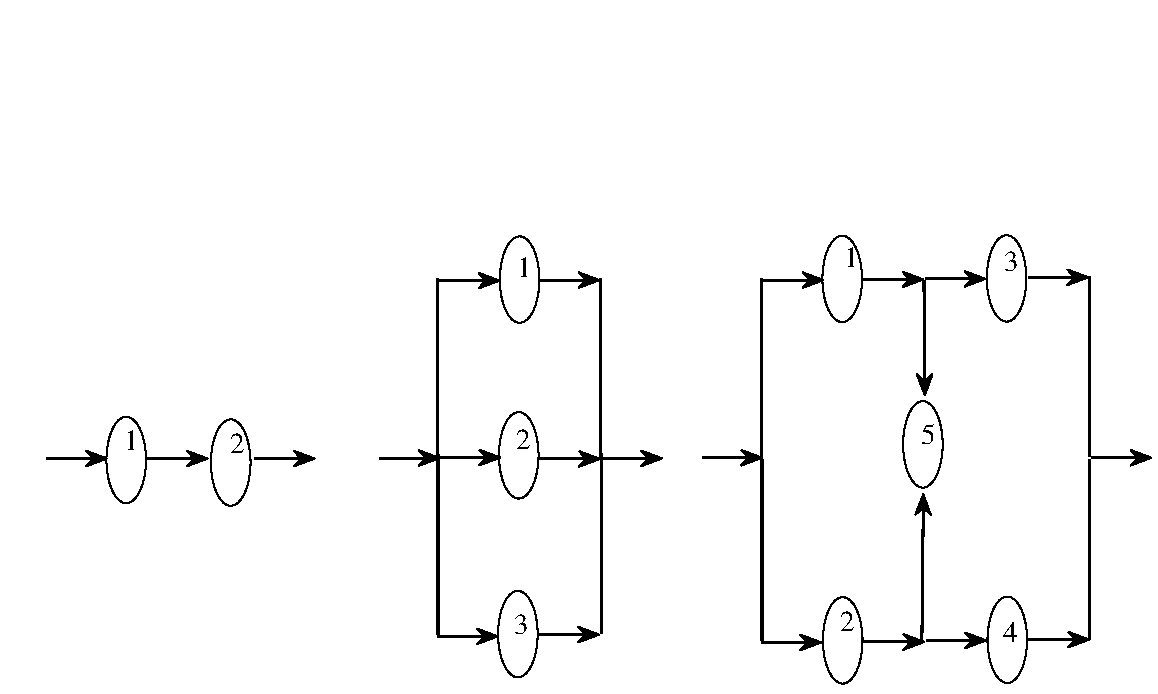
\includegraphics{circuit}
    \caption{Examples of some circuits. \TODO redo}
    \label{fig:circuit}
  \end{marginfigure}
  
  The circuit works if we can enter on the left and leave on the right. Let
  $\omega_i$ be the event that component $i$ works, $p_i=P(\omega_i)$, and $S$
  the even that the system works. Fin d$P(S)$ for the three circuits assuming
  failure of nodes are independent of each other.
  \begin{itemize}
    \item $S=\omega_1 \cap\omega_2$, so $P(S)=P(\omega_1 |\omega_2)P(\omega_2)$.
    By independence, we have $P(S)=P(\omega_1)P(\omega_2)=p_1 p_2$.
    
    \item $S=\omega_1 \cup\omega_2 \cup\omega_3$, so $S'=\omega_1' \cap\omega_2'
    \cap\omega_3'$, and $P(S')=P(\omega_1')P(\omega_2')P(\omega_3')$, hence
    $P(S)=1-(1-p_1)(1-p_2)(1-p_3)$.
    
    \item Let $B_1=\omega_1\cap \omega_3$, $B_2=\omega_2\cap\omega_4$, and
    $B_3=(\omega_1\cap\omega_2'\cap\omega_3'\cap\omega_4\cap\omega_5) \cup 
    (\omega_1'\cap\omega_2'\cap\omega_3'\cap\omega_4'\cap\omega_5')$. $S=B_1\cup
    B_2\cup B_3$, and $B_3\cap B_1=B_3\cap B_2=\emptyset$, and
    $P(S)=P(B_1)+P(B_2)-P(B_1\cap B_2)+P(B_3)$. We see all $\omega_i$ are
    incompatible events, so $P(B_3)=p_1 (1-p_2)(1-p_3)p_4 p_5 + (1-p_1) p_2 p_3
    (1-p_4) p_5$, and hence
    \begin{equation*}
      P(S)=p_1 p_3 + p_2 p_4 - p_1 p_2 p_3 p_4 + P(B_3).
    \end{equation*}
  \end{itemize}
\end{example}

\begin{example}[Example: Hardy--Weinburg equilibrium]
  
  In genetics, offspring get an allele for each gene on a standard chromosome
  from each parent randomly selected from the parents' two alleles and are
  independent. A particular result known as the \Def{Hardy--Weinburg
  equilibrium} states that the ratio of alleles remains constant throughout
  generations, i.e., even dominant genes that confer advantages remain constant
  throughout generations. To see this, it is important to understand what
  happens to neutral alleles, those that do not confer advantages or
  disadvantages.
  
  Suppose for some neutral gene, genotypes $AA$, $Aa$ and $aa$ occur in
  partitions $u$, $2v$ and $w$ respectively ($u+2v+w=1$). Assume that people
  choose mates randomly with respect to this gene and consider the first
  generation of the offspring. Let $AF$, $AM$ be the evens that a given child
  gets allele $A$ from Father and Mother respectively. Let $F_{AA}$, $F_{Aa}$,
  $F_{aa}$ be the evens the Father has the respective genotypes. Using this as a
  partition we get
  \begin{align*}
    P(AF) &= P(AF|F_{AA})P(F_{AA})+P(AF|F_{Aa})P(F_{Aa})+P(AF|F_{aa})P(F_{aa})\\
    &= u+\frac{1}{2}2v+0 = p.
  \end{align*}
  $p=u+v$ denotes the proportion of $A$ alleles and $q=1-p$ denotes the
  proportion of $a$ alleles. The same calculation gives
  \begin{equation*}
    P(AM)=p,\qquad P(aM)=P(aF)=q.
  \end{equation*}
  Then with $C_{AA}$ the event that the child has genotype $AA$ and etc., we
  have
  \begin{align*}
    P(C_{AA}) &= P(AF\cap AM) = p^2,\\ 
    P(C_{aA}) &= P((aF\cap AM)\cup (aM\cap AF)) = qp+pq = 2pq,\\
    P(C_{aa}) &= q^2.
  \end{align*}
  For a large population, the proportions with the various genotypes will be
  close to these probabilities.
  
  Let $u_1 = p^2$, $2v_1=2pq$, $w_1=q^2$ be the proportions in generation 1.
  Proportion of $A$ alleles in generation 2 is
  \begin{equation*}
    u_1+v_1=p^2+pq=p(p+q)=p
  \end{equation*}
  In fact, this is true for $a$ alleles, for all generations. Hence proportion
  of neutral alleles in a population remains constant.
\end{example}

\begin{example}
  The above scenario does not apply to sex-link genes such as $X$ and $Y$
  chromosomes for example. Suppose in an example a gene has alleles $A$ and $a$,
  and $F_{aa}$ and $M_{?a}$ are unhealthy, i.e., men only need an $a$ allele to
  be unhealthy. Suppose Jane is healthy, but has an unhealthy male cousin, but
  all other relatives including two brothers are healthy. Find the probability
  that Jane is of genotype $Aa$, assuming independence.
  
  Let $J$ be the event that Jane is of genotype $Aa$. The father is for sure
  $AA$ since he is healthy; the mother could be either $AA$ or $Aa$. Let $M$ be
  the event that the mother is of genotype $Aa$, and $M'$ the event that the
  mother is of genotype $AA$. Let $B$ the event that both brothers are healthy.
  We want $P(J|B)$; we need $P(J\cap B)$ and $P(B)$. We have, by independence,
  \begin{align*}
    P(B) &= P(B|M)P(M)+P(B|M')P(M')\\
    &=\left(\frac{1}{2}\times\frac{1}{2}\right)\frac{1}{2}+(1\times1)\frac{1}{2}=\frac{5}{8},
  \end{align*}
  and
  \begin{align*}
    P(J\cap B) &= P(J\cap B|M)P(M)+P(J\cap B|M')P(M')\\
    &=\left(\frac{1}{2}\times\frac{1}{2}\times\frac{1}{2}\right)\frac{1}{2} + (0\times1\times1)\frac{1}{2}=\frac{1}{16},
  \end{align*}
  so
  \begin{equation*}
    P(J|B)=\frac{P(J\cap B)}{P(B)}=\frac{1/16}{10/16}=\frac{1}{10}.
  \end{equation*}
\end{example}

%===============================================================================

\section{Random variables, distributions and statistics}

We can now calculate probability for \Def{events}, a collection of
outcomes for some unpredictable trial. We are usually interested in numerical
values based on these outcomes.

For instance, if we throw two dice, there are 36 possible outcomes. Let
\begin{equation*}
  X(\omega) = \omega_1 + \omega_2,
\end{equation*}
where $\omega=(i,j)$ are the values of the respective dices. $X$ here is a
\Def{random variable}. In general, a random variable is a rule for
attaching numerical values to outcomes.

%-------------------------------------------------------------------------------

\subsection{Discrete random variables}

Suppose that $\Omega=\{\omega\}$ is countable, then we say $X$ is a discrete
random variable.
\begin{example}
  Throwing three random coins, we have
  \begin{equation*}
    \Omega=\{HHH, HHT, HTH, HTT, THH, THT, TTH, TTT\}.
  \end{equation*}
  Let $X$ be the number of heads, then $X(1)=1$ for $\omega\in\{TTH, THT,
  HTT\}$. We can use $X=1$ to denote the even that one head shows up, so, in
  this case, $P(X=1) = 3/8$. Similarly, $P(X\geq2) = 1/2$.
\end{example}

For any random variable $X$, the function $p(x) = P(X=x)$ gives us probabilities
for a particular partition of $\Omega$. We call $p(x)$ the
\Def{probability density function} (pdf) of $x$.

We see that $(X=x) \cap (X=y) = \emptyset$ when $x \neq y$, so, by axiom,
\begin{equation*}
  P(x \in A) = \sum_{x\in A}p(x),
\end{equation*}
where $A$ is a set of values. If $X$ takes values in $x_1,x_2,\ldots x_n\ldots$,
then, by axiom,
\begin{equation*}
  \sum_{i\geq 1} p(x_i) = 1.
\end{equation*}

%-------------------------------------------------------------------------------

\subsection{Continuous random variables}

A \Def{continuous} random variable takes values in a continuous set (usually
$\mathbb{R}$ or a subset of it), and has a probability distribution defined by a
non-negative \Def{probability distribution function} (pdf) $f$. We set
\begin{equation*}
  P(X\in A) = \int_A f(x)\, \mathrm{d}x,\qquad A\subseteq\Omega.
\end{equation*}
Generally, $P(a<X<b) = \int_a^b f(x)\, \mathrm{d}x$, and
$\int_{\mathbb{R}}f(x)\, \mathrm{d}x=1$.
\begin{example}
  Suppose we have a pdf
  \begin{equation*}
    f(x) = \begin{cases} k(1+x), & -1<x<0,\\ k(2-x), & 0\leq x<2,\end{cases}
  \end{equation*}
  and zero otherwise. Then
  \begin{equation*}
    1=\int_{-\infty}^\infty f(x)\, \mathrm{d}x = 
    k\int_{-1}^0(1+x)\, \mathrm{d}x + k\int_0^2 (2-x)\, \mathrm{d}x=
    \frac{5k}{2},
  \end{equation*}
  so $k=2/5$.
\end{example}

%-------------------------------------------------------------------------------

\subsection{Binomial distribution}

Suppose there are only two outcomes possible, then, with $n$ trials, there are
$2^n$ outcomes. A particular outcome with $x$ successes has $(n-x)$ failures
associated with it. For $p=P(\textnormal{success})$, the probability of this
outcome is
\begin{equation*}
  p^x (1-p)^{n-x}.
\end{equation*}
Each trial is independent, the event $X=x$ contains many outcomes; in fact,
$C^n_x$ such outcomes. Hence
\begin{equation*}
  P(X=x) = \begin{pmatrix}n\\ x \end{pmatrix} p^x (1-p)^{n-x},\qquad
  x\in[0,n].
\end{equation*}

\begin{example}
  105 people have bought tickets for a flight. They independently miss the
  flight with chance 0.04, so we say $X\sim \mbox{B}(105,0.04)$. Then
  \begin{align*}
    P(X=0) &= 0.96^{105} \approx 0.01376,\\
    P(X=1) &= \begin{pmatrix}105\\ 1\end{pmatrix}(0.04)(0.96)^{104} \approx
    0.06018,
  \end{align*}
  and so on. We also have
  \begin{equation*}
    P(X \geq 3) = \sum_{x=3}^{105} P(x) = 1-\sum_{x=0}^2 P(x) \approx 0.79867.
  \end{equation*}
\end{example}

%-------------------------------------------------------------------------------

\subsection{Poisson distribution}

Suppose events occur randomly at rate $r$ over some time $(t, t+h)$, then
\begin{equation*}
  P(0\ \textnormal{events}) \approx 1-rh,\qquad
  P(1\ \textnormal{event}) \approx rh,\qquad
  P(\geq 2\ \textnormal{events}) \leq h^2,
\end{equation*}
and the number of events in distinct time intervals are independent. The
distribution of the number of events, $T$, in a period of $s$ time units has the
Poisson distribution $T\sim\mbox{Po}(\lambda)$, with parameter $\lambda=rs$. We
can find $P(T=t)$ as a limit of binomial probabilities. Consider an interval of
length $h=s/n$, where $n$ is big and $h$ is small. Let $A_n$ be the even that
all intervals have less than $1$ event. Then
\begin{equation*}
  P(A_n) \geq (1-h^2)^n = \left(1-\frac{sh}{n}\right)^n \to \ex^{-sh}
\end{equation*}
as $n\to\infty$. Note that $\ex^{-sh}\to 1$ as $h\to 0$.

For any fixed $t\in\mathbb{Z}^+$ and for $n>t$,
\begin{align*}
  P(T=t) &\approx P(X_n = t) \\
  &= \begin{pmatrix} n\\ t\end{pmatrix} \left(\frac{\lambda}{n}\right)^t
  \left(1-\frac{\lambda}{n}\right)^{n-t} \\
  &= \frac{n!}{n^t (n-t)!}\frac{\lambda^t}{t!}
  \left(1-\frac{\lambda}{n}\right)^{n-t} \\
  &= \frac{n^{\tilde{t}}}{n^t}\left(1-\frac{\lambda}{n}\right)^{n-t}
  \frac{\lambda^t}{t!},
\end{align*}
where
\begin{equation*}
  \frac{n^{\tilde{t}}}{n^t} = 1\left(1-\frac{1}{n}\right)\cdots
  \left(1-\frac{t-1}{n}\right)\to 1^t=1
\end{equation*}
for $n\to\infty$. So then
\begin{equation*}
  P(T=t)\approx(X_n = t)\to\ex^{-\lambda}\frac{\lambda^t}{t!}
  \qquad(t\in\mathbb{Z}^+)
\end{equation*}
as $n\to\infty$. This limit is an useful approximation for $P(X_n = t)$ with
quite moderate $n$ when $\lambda$ is small. As a rule of thumb, with $p\leq
0.05$, we find that $n=20$ gives a reasonable approximation of the Poisson
distribution to the binomial distribution. With bigger $n$ the approximation is
even better.
\begin{example}
  From 1979 to 1989, 1103 Bristol postmen reported 245 dog biting incidents. 191
  were bitten, 145 of those just once. Are the bites occurring at random or are
  some postmen more prone to dog bites?
  
  Taking each incident as a trial, where each postman has a $1/1103$ chance of
  being attacked. The number of attacks $X$ suffered by a single postman is
  $X\sim\mbox{B}(245,1/1103)$. Hence
  \begin{align*}
    P(X=0) &= \left(1-\frac{1}{1103}\right)^{245}\approx\ex^{-\lambda}, \\
    P(X=1) &= \frac{245}{1103}\left(1-\frac{1}{1103}\right)^{244}\approx
    \lambda\ex^{-\lambda}
  \end{align*}
  with $\lambda=245/1103$. We have that
  \begin{equation*}
    P(X\geq2)\approx0.02,\qquad P(X=0)\approx0.8, \qquad P(X=1)\approx0.18.
  \end{equation*}
  Comparing this to data, we have that
  \begin{align*}
    P(X_{\mbox{data}} = 0) &= \frac{1103-191}{1103} \approx0.83, \\
    P(X_{\mbox{data}} = 1) &= \frac{45}{1103} \approx0.13, \\
    P(X_{\mbox{data}} \geq 2) &\approx 0.04.
  \end{align*}
  Maybe some postmen are more likely to be attacked. We can use a test for
  \Def{goodness of fit}.
\end{example}

%-------------------------------------------------------------------------------

\subsection{Uniform distribution}

Suppose $a<b$, $a,b\in\mathbb{R}$, and $f(x) = 1/(b-a)$ for $x\in(a,b)$ and zero
otherwise. We write the random variable following this probability distribution
by $X\sim \mbox{U}(a,b)$. For $a<c<d<b$, we have
\begin{equation*}
  P(c<X<d) = \frac{d-c}{b-a},
\end{equation*}
while for $c<a<d<b$ (i.e., some of the range lies outside of the support),
\begin{equation*}
  P(c<X<d) = \frac{d-a}{b-a}.
\end{equation*}

%-------------------------------------------------------------------------------

\subsection{Exponential distribution}

Consider some random events occurring at rate $\beta$ (like the Poisson set up).
Let $T$ denote the time to the first event occurring, and consider the event
$\{T>t\} = \{\textnormal{no choices in }(0,t)\}$. We know the probability of no
choices in $(0,t)$, which is
\begin{equation*}
  P(\textnormal{no choices in }(0,t)) = P(X=0) = \ex^{-\beta t},\qquad t>0
\end{equation*}
since $X\sim\mbox{Po}(\beta t)$. Hence, for $t>0$,
\begin{equation*}
  P(T>t) = \ex^{-\beta t},\qquad P(T\leq t) = 1-\ex^{-\beta t},
\end{equation*}
and
\begin{equation*}
  \int_0^x \beta\ex^{-\beta y}\, \mathrm{d}y = 1-\ex^{-\beta x},
\end{equation*}
so $T$ has pdf $f(t) = \beta\ex^{-\beta t}$ for $t>0$. Any random variable with
$X$ with this pdf and $f(t)=0$ for $t<0$ is written $X\sim\mbox{Exp}(\beta)$.

%-------------------------------------------------------------------------------

\subsection{Normal (Gaussian) distribution}

This distribution has two parameters, $\sigma>0$ and $\mu$. We say
$X\sim\mbox{N}(\mu,\sigma^2)$ when its pdf is given by
\begin{equation*}
  f(x) = \frac{1}{\sigma\sqrt{2\pi}}\exp\left[
  -\frac{1}{2}\left(\frac{x-\mu}{\sigma}\right)^2\right]\geq0,
  \qquad x\in\mathbb{R}.
\end{equation*}
This function is symmetric about $\mu$.

%-------------------------------------------------------------------------------

\subsection{Cumulative distribution function (cdf)}

For any random variable $X$, its \Def{cumulative distribution function}
(cdf) is
\begin{equation*}
  F(x) = \begin{cases} \int_{-\infty}^x f(y)\, \mathrm{d}y, & 
  X\ \textnormal{continuous},\\
  \sum_{y\leq x} f(y), & X\ \textnormal{discrete}.\end{cases}
\end{equation*}
The cdf and pdf of $X$ is related by $F'(x) = f(x)$. It is enough to know either
$F$ or $f$ to be able to find $P(X\in A)$ for any set $A$.
\begin{example}
  For the pdf
  \begin{equation*}
    f(x) = \begin{cases}(2/5)(1+y), & -1\leq x<0,\\
    1/5 + (2/5)(2-y), & 0\leq x\leq 2, \end{cases}
  \end{equation*}
  the cdf is
  \begin{equation*}
    F(x) = \begin{cases} 0, & x<-1,\\
    (x+1)^2/5, & -1\leq x < 0,\\
    1-(x-2)/5, & 0\leq x \leq2,\\
    1, & x>2. \end{cases}.
  \end{equation*}
  While $f(x)$ is discontinuous, $F(x)$ is continuous.
\end{example}

\begin{example}
  The standard normal distribution has parameters $\mu=0$, $\sigma=1$. The cdf
  is denoted
  \begin{equation*}
    \Phi(z) = \frac{1}{\sqrt{2\pi}}\int_{-\infty}^z \ex^{-x^2/2}\, \mathrm{d}x,
  \end{equation*}
  and values are tabulated in many books. From symmetry, $\Phi(\mu)=1/2$, and
  $\Phi(-z) = 1-\Phi(z)$. For instance,
  \begin{equation*}
    P(z<-1.04) = 1-\Phi(1.04) = 1 - (0.6\times0.841 + 0.4\times0.864) = 0.150,
  \end{equation*}
  and
  \begin{equation*}
    P(-1.04<z<2.09) = \Phi(2.09)-\Phi(1.04) = 
    (0.1\times0.977 + 0.9\times0.982) - 0.150 = 0.831.
  \end{equation*}
\end{example}

%-------------------------------------------------------------------------------

\subsection{Transformation of random variables}

Suppose $X$ is a random variable and $g:\mathbb{R}\to\mathbb{R}$. Then $g(X)$ is
also a random variable, and is found by composing $g$ with $X$. $X$ assigns
numerical values to trial outcomes, and $g$ transforms this to other numerical
values.
\begin{example}
  Consider $X\sim\mbox{Exp}(\beta)$. Find the distribution of $aX$, $a>0$.
  
  $P(aX\leq y) = P(X\leq y/a) = 1-\ex^{-\beta y/a}$, as $P(X\leq y/a)$ is found
  by the cdf of $aX\sim\mbox{Exp}(\beta)$. Since $aX$ has cdf
  $1-\ex^{-(\beta/a)y}$, $aX\sim\mbox{Exp}(\beta/a)$.
\end{example}

\begin{example}[Example: The probability integral transform]
  Suppose $U\sim\mbox{U}(0,1)$. Consider any random variable $X$ with cdf $F(x)$
  such that it is strictly increasing on $(a,b)$. Hence there exists $F^{-1}$,
  and $F^{-1}$ increases from $a$ to $b$ on $(0,1)$. Consider the distribution
  $F^{-1}(u)$. We have
  \begin{equation*}
    P(F^{-1}(u)\leq X) = P(F(F^{-1}(u)) \leq F(x)) = P(u\leq F(x)),
  \end{equation*}
  so for $X\in(a,b)$, we have $F(x)\in(0,1)$. Thus $P(U\leq F(x)) = F(x)$, and
  hence $F^{-1}(u)$ has the same distribution as $F(u)$.
  
  Suppose $X\sim\mbox{Exp}(\beta)$, so that $F(x) = 1-\ex^{-\beta x}$, $x\geq0$.
  Let $u=1-\ex^{-\beta x}$, so that
  \begin{equation*}
    F^{-1}(u) = -\frac{1}{\beta}\log(1-u),
  \end{equation*}
  and hence $-(1/\beta)\log(1-U)\sim\mbox{Exp}(\beta)$ when
  $U\sim\mbox{U}(0,1)$.
  
  If $X\sim\mbox{N}(\mu,\sigma^2)$ and $Z\sim\mbox{N}(0,1)$, then
  $(X-\mu)/\sigma\sim\mbox{N}(0,1)$, and $\mu+\sigma
  Z\sim\mbox{N}(\mu,\sigma^2)$,
  since
  \begin{equation*}
    \left(\frac{x-\mu}{\sigma}\leq Z\right) \Leftrightarrow
    \left(X\leq \mu+\sigma z\right),
  \end{equation*}
  so that
  \begin{equation*}
    P(X\leq \mu+\sigma z) = P(Z \leq z)
  \end{equation*}
  by letting $z=(x-\mu)/\sigma$.
\end{example}

%-------------------------------------------------------------------------------

\subsection{Discrete jointly distributed random variable}

Suppose $(X,Y)$ takes values $(x_i, y_i)$. The joint pdf of $(X,Y)$ is $P(x_i,
y_i) < P(X=x_i, Y=y_i)$. As before, for any set of outcome pairs $A$, we
calculate
\begin{equation*}
  P((X,Y)\in A) = \sum_{(x,y)\in A} p(x,y).
\end{equation*}
In particular,
\begin{equation*}
  P(X=y) = \sum_y p(x,y) = p_x(x),\qquad
  P(Y=y) = \sum_x p(x,y) = p_y(y),
\end{equation*}
the pdf of $X$ and $Y$ respectively.

\begin{example}
  Suppose that we have two random variables $X$ and $Y$ that are jointly
  distributed, with joint distribution density given by
  \begin{center}
    \begin{tabular}{c|cccc|c}
      $p(x,y)$ & 1 & 2 & 3 & 4 & $p_X(x)$\\
      \hline
      0 & 0 & 0 & 0 & 1/4 & 1/4\\
      1 & 0 & 1/4 & 1/4 & 0 & 1/2\\
      2 & 1/4 & 0 & 0 & 0 & 1/4\\
      \hline
      $p_Y(y)$ & 1/4 & 1/4 & 1/4 & 1/4 & 
    \end{tabular}
  \end{center}
  We see that, in fact, $X\sim\mbox{B}(2,1/2)$ and $Y\sim\mbox{U}(1,4)$.
\end{example}

For any bivarite random variable ($X,Y$), the conditional distribution of $X$
given $Y=y$ is
\begin{equation*}
  P(x|y) = \frac{P(X=x, Y=y)}{P(Y=y)} = \frac{p(x,y)}{p_Y(y)}.
\end{equation*}
Then, for any event $A$ which we describe just using $X$,
\begin{equation*}
  P(A) = \sum_{(x,y)\in A}p(x,y) = \sum_{(x,y)\in A}P(x|y)p_Y(y)
  =\sum_x \sum_y P(x|y)p_Y(y).
\end{equation*}
This is the bivarite version of the partition theorem.

We say $X$ is independent of $Y$ when $P(X=x) = p_X(x) = P(x|y)$, i.e., $p_X(x)
p_Y(y) = p(x,y)$ for all ($x,y$). The previous example is thus not independent.

Consider $g:\mathbb{R}^2\to\mathbb{R}$, so, for example, $X + Y$, $X^2 - Y^2$,
$\ex^{XY}$. Although this can be done, it may be complicated to work out the
joint distribution of $g(X,Y)$.

%-------------------------------------------------------------------------------

\subsection{Continuous jointly distributed random variable}

For a pair $(x,y)$, we describe their probability distribution as the integral
of a joint distribution $f(x,y)$. For any rectangle $[a,b]\times[c,d]$, we
define
\begin{equation*}
  P((x,y)\in A) = \int_a^b \int_c^d f(x,y)\, \mathrm{d}y\, \mathrm{d}x,\qquad
  P(a<x<b) = \int_a^b \int_{-\infty}^\infty f(x,y)\, \mathrm{d}y\, \mathrm{d}x.
\end{equation*}
To obtain marginal densities of $X$ and $Y$, we integrate $f(x,y)$ over the
other variable, i.e.,
\begin{equation*}
  f_X(x) = \int_{-\infty}^\infty f(x,y)\, \mathrm{d}y,\qquad
  f_Y(y) = \int_{-\infty}^\infty f(x,y)\, \mathrm{d}x.
\end{equation*}
Then the \Def{conditional densities} of $X$ given $Y$ is
\begin{equation*}
  f(x|y) =
  \begin{cases}
    f(x,y) / f_Y(y), & f_Y(t) > 0,\\
    0, & f_Y(y) = 0.
  \end{cases}
\end{equation*}
The law of total probability then has a continuous version given by
\begin{equation*}\begin{aligned}
  P(a<x<b) 
    &= \int_a^b \int_{-\infty}^\infty f(x,y)\, \mathrm{d}y\, \mathrm{d}x\\
    &= \int_a^b \int_{-\infty}^\infty f(x|y) f_Y(y)\, \mathrm{d}y\, \mathrm{d}x\\
    &= \int_{-\infty}^\infty \left[ \int_a^b f(x|y)\, \mathrm{d}x \right]
      f_Y(y)\, \mathrm{d}y\\
    &= \int_{-\infty}^\infty P(a<x<b|Y=y) f_Y(y)\, \mathrm{d}y.
\end{aligned}\end{equation*}

\begin{example}
  Suppose $(X,Y)$ has joint density
  \begin{equation*}
    f(x,y) =
      \begin{cases}
        x+y, & (x,y)\in[0,1]^2,\\
        0, & \textnormal{otherwise}.
      \end{cases}
  \end{equation*}
  $f$ is non-negative and is seen to integrate to $1$. The marginal densities
  are then
  \begin{equation*}
    f_X(x) = \int_0^1 f(x,y)\, \mathrm{d}y = x+\frac{1}{2},\qquad
    f_Y(y) = \int_0^1 f(x,y)\, \mathrm{d}x = y+\frac{1}{2}
  \end{equation*}
  for $0 \leq x \leq 1$ and $0 \leq y \leq 1$. We have
  \begin{equation*}
    P\left(\frac{1}{4}<x<\frac{3}{4},\ 0<y<\frac{1}{2}\right) =
    \int_{1/4}^{3/4} \int_0^{1/2} (x+y)\, \mathrm{d}y\, \mathrm{d}x
    =\frac{3}{16},
  \end{equation*}
  \begin{equation*}
    P(X<Y) = \int_0^1 \int_0^y (x+y)\, \mathrm{d}x\, \mathrm{d}y = \frac{1}{2},
  \end{equation*}
  \begin{equation*}
    P(X^2<Y) = \int_0^1 \int_0^{\sqrt{y}} (x+y)\, \mathrm{d}x\, \mathrm{d}y
     = \frac{13}{20},
  \end{equation*}
  and so on. For the conditional probabilities,
  \begin{equation*}
    f(y|x) = \frac{f(x,y)}{f_X(x)} = \frac{x+y}{x+1/2},\qquad
      f(y|x) = \frac{f(x,y)}{f_Y(y)} = \frac{x+y}{y+1/2}.
  \end{equation*}
  We see then $X$ and $Y$ are not independent, since
  \begin{equation*}
    f(x,y) = x+y \neq (x+1/2)(y+1/2) = f_X(x) f_Y(y).
  \end{equation*}
  As a further example, we have
  \begin{equation*}
    P(Y>1/2\ |\ X=x) = \int_{1/2}^1 \frac{x+y}{x+1/2}\, \mathrm{d}y
    = \frac{x+3/4}{2x+1}.
  \end{equation*}
\end{example}

%-------------------------------------------------------------------------------

\subsection{Generating functions}

For any random variable $X$, the function $M_X : \mathbb{R}\to\mathbb{R} \cup
\{\infty\}$ defined by
\begin{equation*}
  M_X (t) = \mathbb{E}\left(\ex^{tX}\right)
\end{equation*}
is called the \Def{moment generation function} of $X$. We have
\begin{equation*}
  M_X(t) =
    \begin{cases}
      \sum_x p(x)\ex^{tx}, & X\ \textnormal{discrete},\\
      \int_{-\infty}^\infty f(x) \ex^{tx}\, \mathrm{d}x, 
        & X\ \textnormal{continuous}.
    \end{cases}
\end{equation*}

\begin{example}
  \begin{enumerate}
    \item If $X\sim\mbox{B}(1,0)$, then
    \begin{equation*}
      M_X(t) = (1-p)\ex^0 + p\ex^{t\cdot1} = p\ex^t + (1-p).
    \end{equation*}
    
    \item If $Y\sim\mbox{Po}(\lambda)$, then
    \begin{equation*}
      M_Y(t) = \ex^{-\lambda}\sum_{k=0}^\infty \frac{(\lambda\ex^{t})^k}{k!}
      = \ex^{\lambda(\ex^{t} - 1)}.
    \end{equation*}
    
    \item If $U \sim \mbox{U}(a,b)$, then
    \begin{equation*}
      M_U(t) = \int_a^b \ex^{tu}\frac{1}{b-a}\, \mathrm{d}u =
      \begin{cases}
        \cfrac{\ex^{bt} - \ex^{at}}{t(b-a)}, & t \neq 0,\\
        1, & t = 0.
      \end{cases}
    \end{equation*}
  \end{enumerate}
\end{example}

Moment generating functions have the following special properties:
\begin{enumerate}
  \item \Def{Moment}. For $r\in\mathbb{Z}^+$,
  \begin{equation*}
    \mathbb{E}(X^r) = \left.\frac{\mathrm{d}^r M_X}{\mathrm{d}t^r}\right|_{t=0}.
  \end{equation*}
  
  \item \Def{Uniqueness}. $M_X(t)$ uniquely determines the probability
  distribution of $f$ provided $M_X(t)$ is finite in $(-h,h)$, $h>0$.
  
  \item \Def{Scaling}. If $X$ has $M_X(t)$ and $Y = aX + b$, then
  \begin{equation*}
    M_Y(t) = \ex^{bt} M_X(at).
  \end{equation*}
  
  \item \Def{Multiplicative}. Suppose $X_1,\ldots X_n$ are independent
  random variables, and let $Y = \sum_{i=1}^n X_i$, then
  \begin{equation*}
    M_Y(t) = \prod_{i=1}^n M_{X_{i}}(t).
  \end{equation*}
  
  \item \Def{Convergence}. Suppose $Y_1,\ldots$ is an infinite sequence of
  random variables, and $Y$ is a further random variable. Suppose $M_Y(t)$ is
  finite for $|t|<a$, $a>0$, and $M_{Y_n}(t) \to M_Y(t)$ as $n \to \infty$ for
  all $t\in(-a,a)$, then
  \begin{equation*}
    P(Y_n \leq c) \to P(Y \leq c)
  \end{equation*}
  as $n\to\infty$ for all $c$ such that $P(Y=c) = 0$.
\end{enumerate}

\begin{example}
  \begin{enumerate}
    \item Suppose $Z\sim\mbox{N}(0,1)$, then
    \begin{align*}
      M_Z(t) 
        & = \frac{1}{\sqrt{2\pi}} \int_{-\infty}^\infty \ex^{tx}\ex^{-x^2/2}\,
          \mathrm{d}x \\
        & = \frac{1}{\sqrt{2\pi}} \int_{-\infty}^\infty
          \ex^{-(x^2 - 2tx + t^2)/2 + t^2/2}\, \mathrm{d}x\\
        & = \frac{\ex^{t^2/2}}{\sqrt{2\pi}} \int_{-\infty}^\infty
          \ex^{(x-t)^2/2}\, \mathrm{d}x\\
        & = \ex^{t^2/2}.
    \end{align*}
    Then we have
    \begin{align*}
      M_Z' (t) = t\ex^{t^2/2} & \qquad\Rightarrow\qquad
      \mathbb{E}(X) = M_Z'(0) = 0,\\
      M_Z''(t) = (t^2 + 1)\ex^{t^2/2} & \qquad\Rightarrow\qquad
      \mbox{Var}(X) = \mathbb{E}(X^2) - [\mathbb{E}(X)]^2 =
      M_Z''(0) - [M_Z'(0)]^2 = 1 - 0 = 1.
    \end{align*}
    
    For general normal distributions, let $W = \sigma Z + \mu$, then
    $W\sim\mbox{N}(\mu\sigma^2)$ and the moment generation function is
    transformed to
    \begin{equation*}
      M_W(t) = \ex^{\mu t}M_Z(\sigma t) = \ex^{\mu t + (\sigma t^2)/2}.
    \end{equation*}
    
    \item Suppose $X_1,\ldots X_n$ are independent and $X_i \sim
    \mbox{Po}(\lambda_i)$ for all $i$. Then
    \begin{equation*}
      M_i(t) = \sum_{x=0}^\infty \ex^{tx} \ex^{-\lambda_i}\frac{\lambda_i^x}{x!}
      = \sum_{x=0}^\infty \ex{-\lambda_i} \frac{(\ex^t \lambda_i)^x}{x!}
      = \ex^{-\lambda_i} \ex^{\lambda_i \ex^t}
      = \ex^{\lambda_i (\ex^t - 1)}.
    \end{equation*}
  \end{enumerate}
\end{example}

Uniqueness implies that $M_Y(t) = \ex^{\lambda (\ex^t -1)}$ iff
$\mbox{Po}(\lambda)$, while $M_Z(t) = \ex^{\mu t + (\sigma t)^2 /2}$ iff
$Z\sim\mbox{N}(\mu,\sigma^2)$. We can show that the sum of Poisson and normal
random variables are still Poisson and normal respectively.

%===============================================================================

\section{Statistics}

%-------------------------------------------------------------------------------

\subsection{Expected values}

For a random variable $X$ we define its \Def{expected value} or
\Def{expectation} $\mathbb{E}(X)$ as
\begin{equation*}
  \mathbb{E}(X) =
    \begin{cases}
      \sum_i x_i p(x_i), & X\ \textnormal{discrete},\\
      \int_{-\infty}^\infty x f(x)\, \mathrm{d}x, & X\ \textnormal{continuous}.
    \end{cases}
\end{equation*}

\begin{example}
  \begin{enumerate}
    \item For $X\sim \mbox{B}(3,1/2)$, $p(x)=1/8,3/8,3/8,1/8$ for $x=0,1,2,3$,
    we have
    \begin{equation*}
      \mathbb{E}(X) = 0\cdot\frac{1}{8} + 1\cdot\frac{3}{8}
        + 2\cdot\frac{3}{8} + 3\cdot\frac{1}{8} = \frac{3}{2}.
    \end{equation*}
    
    \item For $X\sim\mbox{U}(1,n)$, $p(x) = 1/n$, and
    \begin{equation*}
      \mathbb{E}(x) = \frac{1}{n} \sum_i=1^n i = \frac{1}{n}\frac{(n+1)n}{2}
        = \frac{n+1}{2}.
    \end{equation*}
    
    \item $X$ has density $f(x) = x/2$ for $x\in(0,2)$, so
    \begin{equation*}
      \mathbb{E}(X) = \int_0^2 \frac{x^2}{2}\, \mathrm{d}x = \frac{4}{3}.
    \end{equation*}
  \end{enumerate}
\end{example}

We then also have
\begin{equation*}
  \mathbb{E}(g(X)) =
    \begin{cases}
      \sum_{j=1}^\infty p(x_j) g(x_j), & X\ \textnormal{discrete},\\
      \int_{-\infty}^\infty g(x) p(x)\, \mathrm{d}x, & X\ \textnormal{continuous}.
    \end{cases}
\end{equation*}

\begin{example}
  \begin{enumerate}
    \item Suppose $X$ takes integer values between $-2$ and $3$, and $P(X=x) =
    1/6$. Then
    \begin{equation*}
      \mathbb{E}(X^2) = \frac{1}{6}\sum_{x=-2}^3 x^2 = \frac{19}{6},
    \end{equation*}
    and
    \begin{equation*}
      \mathbb{E}(\sin(\pi x/4)) = \frac{1}{6}\left( -1 - \frac{1}{\sqrt{2}} + 0
      + \frac{1}{\sqrt{2}} + 1 + \frac{1}{\sqrt{2}} \right) =
      \frac{1}{6\sqrt{2}}.
    \end{equation*}
    
    \item Suppose $X\sim U(-1,1)$ with $p(x) = 1/2$ and zero otherwise, then
    \begin{equation*}
      \mathbb{E}(X^2) = \frac{1}{2}\int_{-1}^1 x^2\, \mathrm{d}x = \frac{1}{3}.
    \end{equation*}
  \end{enumerate}
\end{example}

Since sums and integrals are linear and additive operations, we see that
\begin{equation*}
  \mathbb{E}(g(X) + h(X)) = \mathbb{E}(g(X)) + \mathbb{E}(h(X))
\end{equation*}
and, as a special case,
\begin{equation*}
  \mathbb{E}(a + bX) = a + b\mathbb{E}(X).
\end{equation*}

%-------------------------------------------------------------------------------

\subsection{Variance}

$\mathbb{E}(X)$ is a description of the average of $X$. We also need a measure
of the spread of $X$'s pdf, and we use the \Def{variance} as it is the
easiest one, defined as
\begin{equation*}
  \mbox{Var}(X) = \mathbb{E}\left([X-\mathbb{E}(X)]^2\right).
\end{equation*}
In applications $\mbox{Var}(X)$ has the wrong units, so we use the
\Def{standard deviation} $\sigma(X)$. By transformation, this is
\begin{equation*}
  \mbox{Var}(X) =
    \begin{cases}
      \sum_{i=1}^\infty (x_i - \mu)^2 p(x_i), & X\ \textnormal{discrete},\\
      \int_{-\infty}^\infty (x_i - \mu)^2 p(x)\, \mathrm{d}x, &
        X\ \textnormal{continuous},
    \end{cases}
\end{equation*}
where $\mu = \mathbb{E}(X)$.

\begin{example}
  \begin{enumerate}
    \item If $X$ takes values $0,10,20$ with $P(X=x) = 1/3$, then
    \begin{equation*}
      \mathbb{E}(X) = 10,\qquad 
      \mbox{Var}(X) = \frac{1}{3}[(0 - 10)^2 + (10 - 10)^2 + (20 - 10)^2]
        \frac{200}{3}.
    \end{equation*}
    
    \item If $X\sim\mbox{N}(0,1)$, then $p(x) = (1/\sqrt{2\pi})\ex^{-x^2/2}$,
    and we notice that $x p(x)$ is an odd function so is has zero mean. On the
    other hand,
    \begin{equation*}
     \mbox{Var}(X) 
      = \frac{1}{\sqrt{2\pi}} \int_{-\infty}^\infty 
        x^2 \ex^{-x^2/2}\, \mathrm{d}x 
      = \frac{1}{\sqrt{2\pi}} \int_{-\infty}^\infty
        x\frac{\mathrm{d}}{\mathrm{d}x}\left(-\ex^{-x^2/2}\right)\, \mathrm{d}x 
      = 1
    \end{equation*}
    after an integration by parts.
  \end{enumerate}
\end{example}

For the variance,
\begin{equation*}
  \mbox{Var}(a+bX) = \mathbb{E}([a+bX - a-b\mathbb{E}(X)]^2) =
    b^2\mathbb{E}([X-\mathbb{E}(X)]^2) = b^2\mbox{Var}(X).
\end{equation*}
Further,
\begin{equation*}
  \mbox{Var}(X) = \mathbb{E}(X^2) - [\mathbb{E}(X)]^2,\qquad
  \mbox{Var}(-X) = (-1)^2 \mbox{Var}(X) = \mbox{Var}(X).
\end{equation*}

%-------------------------------------------------------------------------------

\subsection{Expected values for bivariate random variables}

Suppose $g:\mathbb{R}\to\mathbb{R}^2$, then $g(x,y)$ is a random variable, with
\begin{equation*}
  \mathbb{E}(g(X,Y)) =
    \begin{cases}
      \sum_i \sum_j p(x_i, y_j) g(x_i, y_j), & (X,Y)\ \textnormal{discrete},\\
      \int_{-\infty}^\infty \int_{-\infty}^\infty
        p(x,y) g(x,y)\, \mathrm{d}x\,\mathrm{d}x, & 
        (X,Y)\ \textnormal{continuous}.
    \end{cases}
\end{equation*}

If $(X,Y)$ is a bivariate random variable, with finite $\mathbb{E}(X)$ and
$\mathbb{E}(Y)$, then
\begin{equation*}
  \mathbb{E}(X + Y) = \mathbb{E}(X) + \mathbb{E}(Y).
\end{equation*}

\begin{example}
  \begin{enumerate}
    \item Tickets in a raffle cost 1G. There are 2,000 tickets and some prizes
    totalling 1,000G. Let $X$ denote the amount you win from buying a ticket.
    Every prize is won with a change of $1/2000$, and so we have
    \begin{equation*}
      \mathbb{E}(X_1) = \sum_{i=1}^{2000} \frac{v_i}{2000},
    \end{equation*}
    where $v_i$ is the value of the $i^{\textnormal{th}}$ prize. So
    $\mathbb{E}(X_1) = 1000/2000 = 1/2\textnormal{G}$.
    
    Suppose you buy 20 tickets instead. Let $T = X_1 + \ldots X_{20}$ be the
    total you win. Then $E(T) = E(X_1) + \ldots \mathbb{E}(X_{20}) = 20(1/2) =
    10\textnormal{G}$. We can see that if we buy 2,000 tickets, we recover the
    1,000G, as expected.
    
    \item $X\sim\mbox{B}(n,p)$, and let $S_i = 1$ that trial $i$ is a success
    and $0$ when it is a failure. Then for $X = \sum_i S_i$,
    \begin{equation*}
      \mathbb{E}(X) = \sum_i \mathbb{E}(S_i) = n(1\cdot p + 0\cdot(1-p)) = np.
    \end{equation*}
  \end{enumerate}
\end{example}

%-------------------------------------------------------------------------------

\subsection{Expectation / probability inequalities}

\begin{enumerate}
  \item If a random variable satisfies $X\geq a$, $P(X\geq a) = 1$, then
  $\mathbb{E}(X) \geq a$.
  
  \item For any random variable $X$, $\mbox{Var}(X)\geq0$.
  
  \item \Def{Markov's inequality}: If $P(X\geq0)=1$, then, for $a>0$,
  \begin{equation*}
    P(X\geq a)\leq \frac{\mathbb{E}(X)}{a}.
  \end{equation*}
  This follows because
  \begin{equation*}
    \mathbb{E}(X) = \int_0^\infty xf(x)\, \mathrm{d}x \geq
      \int_a^\infty af(x)\, \mathrm{d}x = aP(X=a)
  \end{equation*}
  for $a>0$.
  
  \item \Def{Chebyshev's inequality}: For any random variable,
  \begin{equation*}
    P(|X-\mathbb{E}(X)| \geq a) \leq \frac{\mbox{Var}(X)}{a^2}.
  \end{equation*}
  To see this, applying Markov's inequality to $[X-\mathbb{E}X]^2$ at $a^2$
  gives
  \begin{equation*}
    P([X-\mathbb{E}(X)]^2\geq a^2) \leq
      \frac{\mathbb{E}([X-\mathbb{E}(X)]^2)}{a^2} = \frac{\mbox{Var}(X)}{a^2},
  \end{equation*}
  and the result follows.
\end{enumerate}

\begin{example}
  If $(X,Y)$ is bivariate with finite $\mathbb{E}(X)$ and $\mathbb{E}(Y)$, then
  shown $\mathbb{E}(Y) \leq \mathbb{E}(X)$ if $P(X\geq Y) = 1$.
  
  Defining $g(X,Y) = X - Y$, we see this is non-negative, so by Markov's
  inequality, $0\leq \mathbb{E}(X-Y) = \mathbb{E}(X) - \mathbb{E}(Y)$, and
  result follows.
\end{example}

Expected values and probabilities are closed related. Consider any set $A$, then
for the characteristic function $\chi_{x\in A}$ (1 if $x\in A$ and 0 otherwise),
we have 
\begin{equation*}
  \mathbb{E}(\chi_{x\in A}) = \sum_i \chi_{x_i \in A}p(x_i)
    = \sum_{x\in A} p(x_i) = P(x\in A).
\end{equation*}

\begin{example}
  Suppose there are 2,000 tickets and 1,000G worth of prizes. Let $X$ denote the
  amount we win with one ticket. By Markov's inequality,
  \begin{equation*}
    P(X\geq 1) \leq \frac{1/2}{1} = \frac{1}{2}.
  \end{equation*}
  Suppose there are 1,000 1G prizes, then $P(X\geq 1) = 1/2$, and by Markov's
  inequality,
  \begin{equation*}
    P(X\geq 1,000) \leq \frac{1/2}{1000} = \frac{1}{2000}.
  \end{equation*}
  Suppose instead there is only one 1,000G prize, then $P(X\geq1000) = 1/2000$.
  This shows the bounds are not sharp.
\end{example}

If $X$ and $Y$ are independent, then $p(x,y) = p_X(x) p_Y(y)$ for all $(x,y)$.
Suppose we can write $f(x,y) = g(x) h(y)$ for all $(x,y)$, then 
\begin{align*}
  \mathbb{E}(f(x,y)) &= \int_{-\infty}^\infty\int_{-\infty}^\infty f(x,y)p(x,y)\, \mathrm{d}x\, \mathrm{d}y \\
    & = \left(\int_{-\infty}^\infty g(x)p_X(x)\, \mathrm{d}x\right)
        \left(\int_{-\infty}^\infty h(y)p_Y(y)\, \mathrm{d}y\right) \\
    & = \mathbb{E}(g(X))\mathbb{E}(h(Y)).
\end{align*}
Further more, $\mathbb{E}(XY) = \mathbb{E}(X)\mathbb{E}(Y)$ if $X$ and $Y$ are
independent.

%-------------------------------------------------------------------------------

\subsection{Conditional expectation}

Suppose $X$ is a discrete variable which takes values in $\Omega$ and suppose
$A\subseteq\Omega$. Then the condition expectation of $X$ given $A$ is
\begin{equation*}
  \mathbb{E}(X\ |\ A) = \sum_{x\in A} xP(X=x\ |\ A).
\end{equation*}

\begin{example}
  Suppose there is a 500G prize and five 100G prizes. Let $A$ be the event we
  win the 500G prize, so $P(X=500\ |\ A) = 1$, so $\mathbb{E}(X\ |\ A) =
  500\cdot1=500$. On the other hand,
  \begin{align*}
    & P(X=5\ |\ A') = \frac{5}{1999}, \qquad P(X=0\ |\ A') = \frac{1994}{1999},\\
    \Rightarrow \qquad & \mathbb{E}(X=x\ |\ A') = 100\cdot\frac{5}{1999} = \frac{500}{1999}.
  \end{align*}
\end{example}

\begin{theorem}[Partition theorem]
  If events $A_1,\ldots A_n$ form a partition of $\Omega$, then
  \begin{equation*}
    \mathbb{E}(X) = \sum_{i=1}^n \mathbb{E}(X\ |\ A_i) P(A_i).
  \end{equation*}
\end{theorem}
\begin{proof}
  Suppose $X$ has possible values $x_i,\ldots x_k\ldots$. By definition of
  $\mathbb{E}(X)$ and the partition theorem,
  \begin{equation*}
    \mathbb{E}(X) = \sum_{j=1}^\infty x_j P(X=x) 
    = \sum_{j=1}^\infty x_j \sum_{i=1}^n P(X=x_j\ |\ A_i)P(A_i).
  \end{equation*}
  Re-arranging the order of summation,
  \begin{equation*}
    \mathbb{E}(X) = 
      \sum_{i=1}^n \left(\sum_{j=1}^\infty x_jP(X=x_j\ |\ A_i)\right)P(A_i)
    = \sum_{i=1}^n E(X\ |\ A_i) P(A_i).
  \end{equation*}
  \qed
\end{proof}

\begin{example}
  With the above example,
  \begin{equation*}
    \mathbb{E}(X) = 500\cdot\frac{1}{2000} + \frac{500}{1999}\frac{1999}{2000}
    = \frac{1}{2}.
  \end{equation*}
\end{example}

Consider a bivarite random variable $(X,Y)$, and we seek $\mathbb{E}(X\ |\
Y=y)$. The conditional probability $P(X=x\ |\ A)$ is denoted by $p(x\ |\ y)$,
hence
\begin{equation*}
  \mathbb{E}(X\ |\ Y=y) =
  \begin{cases}
    \sum_x xp(x\ |\ y), & (x,y)\ \textnormal{discrete},\\
    \int_{-\infty}^\infty xp(x\ |\ y)\, \mathrm{d}x, & (x,y)\
    \textnormal{continuous}.
  \end{cases}
\end{equation*}
We can write $g(y) = \mathbb{E}(X\ |\ Y=y)$, and here
\begin{equation*}
  \mathbb{E}(g(Y)) = \sum_y p_Y(y) g(y) = \mathbb{E}(X),
  \qquad\Rightarrow\qquad
  \mathbb{E}(\mathbb{E}(X\ |\ Y)) = \mathbb{E}(X).
\end{equation*}
This is because
\begin{align*}
  \mathbb{E}(\mathbb{E}(X\ |\ Y)) & = \sum_y p_Y(y) g(y) \\
    &= \sum_y p_Y(y) \left(\sum_x xp(x\ |\ y)\right) \\
    &= \sum_x x \sum_y p_Y(y) p(x\ |\ y) \\
    &= \sum_x \sum_y p(x,y) \\
    &= \sum_x p_X(x) = \mathbb{E}(X).
\end{align*}

\begin{example}
  A shop gets $N$ customers a day, with $\mathbb{E}(N) = 800$. Each customer
  independently spends $X_i$, with $\mathbb{E}(X_i) = 25$. Let $T = \sum_{i=1}^n
  X_i$ be the amount of turnover of the shop in the day. Taking a partition of
  $N$, we know that
  \begin{equation*}
    \mathbb{E}(T\ |\ N=n) = \sum_{i=1}^n \mathbb{E}(X_i\ |\ N=n) =
    \sum_{i=1}^n \mathbb{E}(X_i) = 25n.
  \end{equation*}
  So then
  \begin{align*}
    \mathbb{E}(T) &= \sum_{n=1}^\infty \mathbb{E}(T\ |\ N=n) P(N=n) \\
      &= \sum_{n=1}^\infty 25n p(N=n) \\
      &= 25 \sum_{n=1}^\infty np(N=n) \\
      &= 25\mathbb{E}(N) = 20000,
  \end{align*}
  which we would have expected from intuition anyway.
\end{example}

%-------------------------------------------------------------------------------

\subsection{Co-variance}

Suppose $X$ and $Y$ are jointly distributed random variables. Then the
co-variance of $X$ and $Y$ is
\begin{equation*}
  \mbox{Cov}(X,Y) = \mathbb{E}([X - \mathbb{E}(X)][Y - \mathbb{E}(Y)]).
\end{equation*}
This can be re-written as
\begin{equation*}
  \mbox{Cov}(X,y) = \mathbb{E}(XY) - \mathbb{E}(X)\mathbb{E}(Y).
\end{equation*}

\begin{example}
  \begin{align*}
    \mbox{Var}(X+Y) 
      & = \mathbb{E}\left( [(X+Y) - \mathbb{E}(X+Y)]^2\right) \\
      & = \mathbb{E}\left([(X-\mathbb{E}(X))^2 + (y-\mathbb{E}(Y))^2]\right) \\
      & = \mathbb{E}\left( [X-\mathbb{E}(X)]^2 +
        2\mathbb{E}([X-\mathbb{E}(Y)][Y-\mathbb{E}(X)])
        +[Y-\mathbb{E}(Y)]^2\right)\\
      & = \mbox{Var}(X) + 2\mbox{Cov}(X,Y) + \mbox{Var}(Y).
  \end{align*}
\end{example}

Some properties of the co-variance:
\begin{enumerate}
  \item For all $X$, $\mbox{Var}(X) = \mbox{Cov}(X,X)$.
  \item For all $X$ and $Y$, $\mbox{Cov}(X,Y) = \mbox{Cov}(Y,X)$.
  \item For all $X$, $Y$ and $Z$,
  \begin{align*}
    \mbox{Cov}(aX, bY) & = ab\mbox{Cov}(X,Y),\\
    \mbox{Cov}(X+Y, Z) & = \mbox{Cov}(X,Z) + \mbox{Cov}(Y,Z),\\
    \mbox{Cov}(X, Y+Z) & = \mbox{Cov}(X,Y) + \mbox{Cov}(X,Z).
  \end{align*}
  \item If $X$ and $Y$ are independent, $\mbox{Cov}(X,Y) = 0$.
\end{enumerate}

\begin{example}
  $n$ people throw their hats up and catch it. Let $H$ be the event the person
  catches their own hat. $H$ is not binomial as trials are not independent. Let
  $X_i = 0$ if person $i$ catches someone else's hat, and $1$ is person $i$
  catches their own hat. Then $H = \sim_{i=1}^n X_i$. We know that
  \begin{equation*}
    \mathbb{E}(X_i)^p = \frac{1}{n} \cdot 1^p + \frac{n-1}{n} \cdot 0^p
    = \frac{1}{n},
  \end{equation*}
  so then $\mathbb{E}(H) = \sum_{i=1}^n X_i = n/n = 1$. We also have
  \begin{align*}
    \mbox{Var}(H) 
      & = \sum_{i=1}^n \mbox{Var}(X_i) + 2\sum_{i<j}\mbox{Cov}(X_i, X_j), \\
    \mbox{Var}(X_i) 
      & = \mathbb{E}(X_i^2) - \left[\mathbb{E}(X_i)\right]^2
      \frac{1}{n} - \frac{1}{n^2}, \\
    \mbox{Cov}(X_i, X_j) 
      & = \mathbb{E}(X_i X_j) - \mathbb{E}(X_i)\mathbb{E}(X_j), \\
    \mathbb{E}(X_i, X_j) 
      & = 1\cdot P(X_i = 1, X_j = 1) = P(X_i = 1\ |\ X_j = 1)P(X_j = 1)
        = \frac{1}{n-1}\frac{1}{n}.
  \end{align*}
  Together, this gives
  \begin{equation*}
    \mbox{Var}(H) = \frac{1}{n} - \frac{1}{n^2} +
      2\frac{n(n-1)}{2}\frac{1}{n^2 (n-1)} = 1
  \end{equation*}
\end{example}

\begin{example}
  For $X\sim\mbox{B}(n,p)$, $X = X_i + \ldots X_n$, with $\mathbb{E}(X) = np$.
  For each trial $i$,
  \begin{equation*}
    \mbox{Var}(X_i) = \mathbb{E}(X_i^2) - p^2 =
    1^2\cdot p + 0^2(1-p) - p^2 = p(1-p).
  \end{equation*}
  Each trial is independent so $\mbox{Var}(X) = \sum_{i=1}^n \mbox{Var}(X_i) =
  np(1-p)$.
  
  For $X\sim\mbox{B}(n,1/n)$,
  \begin{equation*}
    \mbox{Var}(X) = n\frac{1}{n}\left(1-\frac{1}{n}\right) = 
    \left(1-\frac{1}{n}\right).
  \end{equation*}
  For large $n$, $H$ (from the previous example) and $X$ are approximately
  follows a Poisson distribution with $\lambda = 1$.
  
  Chebyshev's inequality says that $P(|X-\mathbb{E}(X)| \geq t) \leq
  \mbox{Var}(X) / t^2$, so for $X\sim\mbox{B}(n,p)$ with $t=n\epsilon$, we have
  \begin{equation*}
    P(|X - np| \geq n\epsilon) \leq \frac{np(1-p)}{n^2\epsilon^2}
    = \frac{p(1-p)}{\epsilon^2}\frac{1}{n}.
  \end{equation*}
\end{example}


%===============================================================================

\section{Limit theorems}

%-------------------------------------------------------------------------------

\subsection{Stability of sample proportion}

Suppose $X\sim\mbox{B}(n,p)$ and $B_n = X/n$, which is the proportion of trials
that are successes. We know that $\mathbb{E}(X) = np$ and $\mbox{Var}(X) =
np(1-p)$ from the previous example. So from the properties of the expectation
and the variance,
\begin{equation*}
  \mathbb{E}(B_n) = \frac{1}{n}\mathbb{E}(X) = p,\qquad
  \mbox{Var}(B_n) = \frac{\mbox{Var}(X)}{n^2} = \frac{p(1-p)}{n}.
\end{equation*}
By Chebyshev's inequality,
\begin{equation*}
  P(|B-n - p| \geq \epsilon) \leq \frac{p(1-p)}{\epsilon^2} \frac{1}{n}
  \to 0
\end{equation*}
as $n\to\infty$ for all $t$. So that \emph{$n\to\infty$, the sample
proportion is within a small interval centred on $p$, the expected value of the
trial}.

%-------------------------------------------------------------------------------

\subsection{Law of large numbers}

Let $X_1,\ldots X_n$ are $n$ trials on some experiment that we know are
independent, and $\mathbb{E}(X_i) = \mu$ and $\mbox{Var}(X_i) = \sigma^2$ for
all $i$. Considering $\overline{X_n}$, the sample mean random variable, then
\begin{align*}
  \mathbb{E}(\overline{X_n}) 
    & = \frac{1}{n}\mathbb{E}\left(\sum_{i=1}^n X_i\right) \frac{n\mu}{\nu} 
    = \mu,\\
  \mbox{Var}(\overline{X_n}) 
    & = \frac{1}{n^2}\mbox{Var}\left(\sum_{i=1}^n X_i\right)
    = \frac{n\sigma^2}{n^2} = \frac{\sigma^2}{n}.
\end{align*}
Hence, by Chebyshev's inequality, for all $t > 0$, 
\begin{equation*}
  P(|\overline{X_n} - \mu|\geq t) \leq \frac{\sigma^2}{nt^2} \to 0
\end{equation*}
as $n\to\infty$. So \emph{the average random variable has a high probability of
being near to $\mu$ for large $n$}.

%-------------------------------------------------------------------------------

\subsection{Normal approximation to binomial}

If $X\sim\mbox{B}(n,p)$, with $n$ large and $p$ not near $0$ or $1$, then $X$ is
approximately $\mbox{N}(np, np(1-p))$. Then, for any $c$,
\begin{equation*}
  P(X\leq c)\approx \Psi\left(\frac{c-\mu}{\sigma}\right) =
  \Psi\left(\frac{c-np}{\sqrt{np(1-np)}}\right).
\end{equation*}
\begin{example}
  A student must scale more than $30$ on a multiple choice test with $n=50$
  questions. Suppose he has $p=1/2$ change of answering correctly. Let $X$ be
  the number of correct answers, so $X\sim\mbox{B}(50,1/2)$, and we wish to
  estimate $P(X\geq30) = 1 - P(X\leq 29) = 1 - P(X < 30)$. Using a continuity
  correction of $c=29.5$ gives
  \begin{align*}
    P(X \geq 30) & \approx 1 - \Phi\left(\frac{29.5 - \mu}{\sigma}\right) \\
      &= 1 - \Phi(1.273) = 0.102 \qquad \left(\mu=25,\quad \sigma^2 = \frac{25}{2}\right).
  \end{align*}
\end{example}

%-------------------------------------------------------------------------------

\subsection{Central Limit Theorem (CLT)}

Suppose we have a sequence of random variables $X_1,\ldots$ with
$\mathbb{E}(X_i) = \mu$, $\mbox{Var}(X_i) = \sigma^2$ for all $i$. Let $S_n =
\sum_{i=1}^n X_i$, then $\mathbb{E}(S_n) = n\mu$, $\mbox{Var}(S_n) = n\sigma^2$.
For large $n$, $S_n \sim \mbox{N}(n\mu, n\sigma^2)$, i.e.,
\begin{equation*}
  Z_n = \frac{S_n - n\mu}{\sigma\sqrt{n}} 
  = \frac{1}{\sqrt{n}}\sum_{i=1}^n \frac{X_i - \mu}{\sigma}.
\end{equation*}
Then $P(Z_n \leq c) \to \Phi(c)$ as $n\to\infty$. For any set of $n$ numbers the
difference between their total $t$ and their average $\overline{x}$ is expressed
by $\overline{x} = t/n$.

CLT also applies to the sample average $\overline{X} = n^{-1} \sum_{i=1}^n X_i$.
A useful form of the approximation is
\begin{equation*}
  P(\overline{X} \leq \mu + c\sigma/\sqrt{n}) \approx \Phi(c).
\end{equation*}

\begin{example}
  Measures from an experiment have mean $\mu$ and $\sigma = 2.5$. Find the $n$
  such that $P(|\overline{X_n} - \mu| \leq 0.1) \geq 0.95$.
  
  We know that
  \begin{equation*}
    \mathbb{E}(\overline{X_n}) = \mathbb{E}\left(\frac{1}{n}S_n\right)
    = \frac{n\mu}{n} = \mu,\qquad
    \mbox{Var}(\overline{X_n}) = \mbox{Var}\left(\frac{1}{n}S_n\right)
    = \frac{n\sigma^2}{n^2} = \frac{\sigma^2}{n}.
  \end{equation*}
  With $P(\overline{X} \leq \mu + c\sigma/\sqrt{n}) \approx \Phi(c)$, we have
  \begin{equation*}
    P(|\overline{X_n} - \mu| \leq c\sigma/n) \approx \Phi(c) - \Phi(-c),
    \qquad c > 0.
  \end{equation*}
  So we need $c\sigma/n \leq 0.1$, $\Phi(c) - \Phi(-c) > 0.95$. Choosing $c =
  1.96 \approx 2$, this gives
  \begin{equation*}
    0.1 \leq \frac{2.5(2\sigma)}{\sqrt{n}} \qquad\Rightarrow\qquad
    \sqrt{n} \geq 50 \qquad\Leftrightarrow\qquad
    n \geq 2,500.
  \end{equation*}
\end{example}

%===============================================================================

%%%%%%%%%%%%%%%%%%%%%%%%%%%%%%%%%%%%%%%%%

% r.5 contents
%\tableofcontents

%\listoffigures

%\listoftables

% r.7 dedication
%\cleardoublepage
%~\vfill
%\begin{doublespace}
%\noindent\fontsize{18}{22}\selectfont\itshape
%\nohyphenation
%Dedicated to those who appreciate \LaTeX{} 
%and the work of \mbox{Edward R.~Tufte} 
%and \mbox{Donald E.~Knuth}.
%\end{doublespace}
%\vfill

% r.9 introduction
% \cleardoublepage

%%%%%%%%%%%%%%%%%%%%%%%%%%%%%%%%%%%%%%%%%
% actual useful crap (normal chapters)
\mainmatter

%\part{Basics (?)}


%\backmatter

%\bibliography{refs}
\bibliographystyle{plainnat}

%\printindex

\end{document}

